\documentclass[11pt,letterpaper]{article}
\usepackage[margin=0.83in,headheight=14pt]{geometry}
\usepackage[T1]{fontenc}
\usepackage{newtxtext}
\usepackage{amsmath,amssymb,mathtools,booktabs,array,tabularx,microtype,enumitem,xcolor,fancyhdr,lastpage,graphicx,caption,pgfplots}
\usepackage{newtxmath}
\usepackage[hidelinks]{hyperref}
\pgfplotsset{compat=1.18}
\usetikzlibrary{positioning}
\usepgfplotslibrary{fillbetween}
\definecolor{ink}{HTML}{173C55}
\definecolor{muted}{HTML}{52616A}
\definecolor{accent}{HTML}{237B78}
\usepackage{titlesec}
\titleformat{\section}{\large\bfseries\color{ink}}{\thesection.}{0.55em}{}
\titleformat{\subsection}{\normalsize\bfseries}{\thesubsection.}{0.5em}{}
\titlespacing*{\section}{0pt}{12pt}{6pt}
\titlespacing*{\subsection}{0pt}{9pt}{4pt}
\setlength{\parindent}{0pt}
\setlength{\parskip}{5pt plus 1pt}
\setlength{\abovedisplayskip}{6pt plus 2pt minus 2pt}
\setlength{\belowdisplayskip}{6pt plus 2pt minus 2pt}
\setlist{nosep,leftmargin=1.35em}
\captionsetup{font=small,labelfont=bf,skip=5pt,hypcap=false}
\pagestyle{fancy}
\fancyhf{}
\fancyhead[L]{\small\color{muted}Task-aware amortized importance sampling}
\fancyhead[R]{\small\color{muted}Research proposal}
\fancyfoot[C]{\small\thepage\ / \pageref{LastPage}}
\renewcommand{\headrulewidth}{0.4pt}
\newcommand{\E}{\mathbb E}
\newcommand{\R}{\mathbb R}
\newcommand{\N}{\mathcal N}
\newcommand{\norm}[1]{\lVert #1\rVert_2}
\newcommand{\ESS}{\operatorname{ESS}}
\newcommand{\MSE}{\operatorname{MSE}}
\newcommand{\KL}{D_{\mathrm{KL}}}
\newcommand{\dev}{K_{\mathrm{dev}}}
\newcommand{\task}{\mathrm{task}}
\newcolumntype{Y}{>{\raggedright\arraybackslash}X}
\begin{document}
\begin{center}
{\LARGE\bfseries\color{ink} Task-Aware Amortized Importance Sampling\par}
\vspace{5pt}
{\large From asymptotic difficulty to finite-sample risk under fixed sampling budgets\par}
\vspace{9pt}
{\normalsize Pujan Avaiya\par}
\vspace{3pt}
{\small Research proposal with completed preliminary studies\par}
\end{center}
\vspace{3pt}

\begin{abstract}
\noindent Importance sampling estimates posterior quantities when direct posterior sampling is difficult. In a batch of observations, uniform allocation and weight-based diagnostics do not explicitly minimize error for a specified posterior statistic. I study a learned allocation method based on the asymptotic variance of self-normalized importance sampling (SNIS), using an offline Monte Carlo teacher and a gradient-boosted regressor. On 25 independent test datasets per dimension, the original 4D and 8D Gaussian-mixture experiments gave 10.16\% and 8.92\% lower posterior-mean MSE than uniform allocation. A follow-up on 25 further datasets per dimension reproduced the gain (10.45\% and 8.88\%), but simple context-noise rules performed better (11.90\% and 10.25\%). Even the exact integer-constrained asymptotic oracle achieved only 6.50\% and 5.48\% measured reductions. Across 300 observations per dimension, at 48 draws the empirical risk was 57.7\% and 49.7\% of its asymptotic approximation. The variance nevertheless retained useful ranking information. Transfer to variational autoencoders (VAEs) was less convincing: independent Hamiltonian Monte Carlo (HMC) references gave an inconclusive 0.495\% reduction in 8D. These findings motivate a narrower question: can a learned finite-sample risk model improve over inexpensive allocation rules, and can calibration identify when the learned allocation should be shrunk toward a reliable baseline?
\end{abstract}
\section{Research problem and motivation}
In a probabilistic generative model, an observed variable $x$ is related to an unobserved latent variable $z$ through $p_\theta(x,z)=p(z)p_\theta(x\mid z)$. Bayesian inference asks which latent values are plausible given $x$. For nonlinear models, normalizing $p_\theta(z\mid x)$ is generally intractable. Importance sampling provides a way to estimate posterior expectations using an accessible proposal distribution.

The computational problem is how to distribute a fixed number of importance samples across a batch. Uniform allocation ignores differences in inference difficulty; effective sample size (ESS) measures weight concentration but not the error of the chosen statistic. A learned predictor might estimate difficulty without test-time pilot sampling, but learning is useful only if it adds information beyond readily available features such as observation noise and proposal width.

\textbf{Central research question.} Under a fixed online sampling budget, when does a learned, task-specific allocation improve finite-sample posterior-mean estimation over simple rules, and when should we trust or shrink its predictions?

The project originated in undergraduate research; the expanded experiments and audits reported here are subsequent follow-up work conducted in 2026. The aim is not to change the posterior or improve VAE reconstruction, but to allocate computation for inference with a fixed generative model. The completed studies establish the motivation for the proposed research; the new finite-sample learning and reliability-aware experiments in Section~\ref{sec:future} are not yet completed.
\clearpage
\section{Mathematical foundations}
\subsection{Posterior expectations and self-normalized importance sampling}
Let $x_i$ denote observation $i$, $p_i(z)=p_\theta(z\mid x_i)$ the target posterior, and $q_i(z)$ an accessible proposal whose support covers the target. Define the unnormalized weight and marginal likelihood
\begin{equation}
 w_i(z)=\frac{p_\theta(x_i,z)}{q_i(z)},\qquad Z_i=p_\theta(x_i)=\E_{q_i}[w_i(z)].
 \label{eq:weights}
\end{equation}
For a function $h:\R^d\to\R^m$, the posterior quantity of interest is $\mu_i=\E_{p_i}[h(z)]$. Since $p_i/q_i=w_i/Z_i$,
\begin{equation}
 \mu_i=\frac{\E_{q_i}[w_i(z)h(z)]}{\E_{q_i}[w_i(z)]}.
\end{equation}
Given $K_i$ independent proposal draws $z_{ik}\sim q_i$, self-normalized importance sampling (SNIS) estimates this quantity by
\begin{equation}
 \widehat\mu_{i,K_i}=\frac{\sum_{k=1}^{K_i}w_i(z_{ik})h(z_{ik})}{\sum_{k=1}^{K_i}w_i(z_{ik})}
 =\sum_{k=1}^{K_i}\widetilde w_{ik}h(z_{ik}),\qquad
 \widetilde w_{ik}=\frac{w_i(z_{ik})}{\sum_{\ell=1}^{K_i}w_i(z_{i\ell})}.
 \label{eq:snis}
\end{equation}
The ratio estimator is generally biased at finite $K_i$, but is consistent under standard support and integrability assumptions. Throughout the main experiments $h(z)=z$, so $\mu_i$ is the posterior mean vector.
\subsection{Derivation of task-specific asymptotic variance}
For clarity, suppress the observation subscript and let $K$ be the number of draws. Subtracting $\mu$ from Eq.~\eqref{eq:snis} gives the exact identity
\begin{equation}
 \sqrt K(\widehat\mu_K-\mu)=\frac{K^{-1/2}\sum_{k=1}^{K}w(z_k)[h(z_k)-\mu]}{K^{-1}\sum_{k=1}^{K}w(z_k)}.
\end{equation}
The numerator is a sum of centered independent random vectors, because $\E_q[w(h-\mu)]=Z\mu-Z\mu=0$. If its second moment is finite, the multivariate central limit theorem applies. The denominator converges almost surely to $Z>0$ by the law of large numbers. Slutsky's theorem yields
\begin{align}
 \sqrt K(\widehat\mu_K-\mu)&\xrightarrow{d}\N(0,\Gamma_h),\\
 \Gamma_h&=\E_q\!\left[\left(\frac{w(z)}{Z}\right)^2(h(z)-\mu)(h(z)-\mu)^\top\right].
\end{align}
The trace of the covariance defines a scalar task-specific difficulty:
\begin{equation}
 \boxed{\tau_{i,h}^{2}=\operatorname{tr}(\Gamma_{i,h})=\E_{q_i}\!\left[\left(\frac{p_i(z)}{q_i(z)}\right)^2\norm{h(z)-\mu_i}^2\right].}
 \label{eq:tau}
\end{equation}
With additional moment conditions sufficient for convergence of second moments, the leading squared-error risk is
\begin{equation}
 \E\norm{\widehat\mu_{i,K_i}-\mu_i}^2\approx\frac{\tau_{i,h}^{2}}{K_i}.
 \label{eq:risk}
\end{equation}
This expression accounts for both proposal--posterior mismatch and the influence of a latent sample on the chosen statistic. A high-weight sample close to the mean has a different contribution from a high-weight sample far from it. For $h(z)=z$ we write $\tau_i=\tau_{i,h}$. Dividing the risk by $d$ gives the per-coordinate MSE used in the experiments; the common factor does not affect the optimal allocation within a dimension.

Equation~\eqref{eq:risk} is an asymptotic approximation, not a finite-budget guarantee. In particular, light-tailed proposals can violate the moment conditions; even when they hold, the online budget of approximately 48 samples per observation may not be in the asymptotic regime.
\clearpage
\subsection{Why ESS is not a task-specific difficulty measure}
The conventional empirical ESS of $K_i$ importance samples is
\begin{equation}
 \widehat{\ESS}_i=\frac{(\sum_k w_{ik})^2}{\sum_k w_{ik}^2}=\frac{1}{\sum_k\widetilde w_{ik}^{\,2}}.
\end{equation}
Writing $r_i=p_i/q_i$, the limiting ESS fraction is $1/\E_{q_i}[r_i^2]$ when the relevant moments exist. It does not include $h(z)$, whereas Eq.~\eqref{eq:tau} contains $\norm{h(z)-\mu_i}^2$. For an explicit counterexample, take exact proposals $q_1=p_1=\N(0,0.01)$ and $q_2=p_2=\N(0,9)$, with $h(z)=z$. Both have constant weights and $\widehat{\ESS}_i=K_i$. Their posterior standard deviations are nevertheless $0.1$ and $3$, so their mean-estimation variances at equal $K_i$ differ by a factor of 900. ESS alone cannot distinguish these tasks.
\subsection{Optimal continuous allocation under a fixed budget}
Let $a_i>0$ denote the relative importance of observation $i$ and let $B$ be the total sample budget. For equal sample-evaluation costs, the idealized objective is
\begin{equation}
 \min_{K_i>0}\ J(K)=\sum_{i=1}^n\frac{a_i\tau_i^2}{K_i},\qquad \sum_{i=1}^n K_i=B.
 \label{eq:opt}
\end{equation}
Assume $\tau_i>0$. The Lagrangian is $\mathcal L=J+\lambda(\sum_i K_i-B)$. The first-order conditions are $-a_i\tau_i^2/K_i^2+\lambda=0$, giving $K_i=\sqrt{a_i}\tau_i/\sqrt\lambda$. The budget condition determines $\sqrt\lambda=\sum_j\sqrt{a_j}\tau_j/B$. Therefore,
\begin{equation}
 \boxed{K_i^*=B\frac{\sqrt{a_i}\tau_i}{\sum_j\sqrt{a_j}\tau_j}.}
 \label{eq:optimal}
\end{equation}
Since $\partial^2 J/\partial K_i^2=2a_i\tau_i^2/K_i^3>0$, the stationary point is the unique global minimum of the continuous problem. For equal observation weights, the allocation is proportional to the standard-deviation score $\tau_i$, not to $\tau_i^2$. In that case, Cauchy--Schwarz gives
\begin{equation}
 J^*=\frac{(\sum_i\tau_i)^2}{B}\leq \frac{n}{B}\sum_i\tau_i^2=J_{\mathrm{uniform}}.
\end{equation}
Equality holds when all $\tau_i$ are equal. Thus there is little theoretical room for adaptive allocation if inference difficulties are nearly homogeneous.
\subsection{Sensitivity to learned difficulty errors}
The optimal policy assumes that $\tau_i$ is known. If $s_i>0$ is a prediction, let $b_i=s_i/\sum_j s_j$ and $b_i^*=\tau_i/\sum_j\tau_j$. For equal weights and unrestricted continuous allocation, substituting $K_i=Bb_i$ into Eq.~\eqref{eq:opt} yields
\begin{equation}
 \frac{J(Bb)}{J^*}=\sum_i\frac{(b_i^*)^2}{b_i}=1+\sum_i\frac{(b_i-b_i^*)^2}{b_i}.
 \label{eq:regret}
\end{equation}
The last equality follows from $\sum_i b_i=\sum_i b_i^*=1$. It explains why underallocating a difficult observation can be particularly costly and why ranking accuracy alone may not be sufficient. This identity concerns the asymptotic objective only. Its relationship to finite-sample risk must be tested rather than assumed.

\clearpage
\section{Original learning-based allocation method}
\subsection{Offline teacher estimates}
The quantity in Eq.~\eqref{eq:tau} is unknown for a new observation. A pilot can estimate difficulty at test time, but its draws consume part of the inference budget. The original method estimates difficulty on development observations and trains a supervised regressor; Section~\ref{sec:baselines} tests the cost of a pilot explicitly. For each development observation, draw $M=\dev$ samples from its proposal and calculate the normalized weights and teacher posterior mean $\widetilde\mu_i=\sum_k\widetilde w_{ik}z_{ik}$. Replacing the expectation and normalizer in Eq.~\eqref{eq:tau} by their sample counterparts gives
\begin{equation}
 \widehat\tau_i^2=M\sum_{k=1}^{M}\widetilde w_{ik}^{\,2}\norm{z_{ik}-\widetilde\mu_i}^2.
 \label{eq:teacher}
\end{equation}
The synthetic implementation uses $s_i^{\task}=\sqrt{\max(\widehat\tau_i^2,10^{-5})+0.02}$ and $s_i^{\mathrm{ESS}}=\sqrt{\max(M/\widehat{\ESS}_i-1,0)+0.05}$. These are finite-sample proxies, not exact labels; the positive offsets stabilize the allocation. The later VAE code uses offsets outside the square roots. The same synthetic teacher convention is retained in the new comparisons.
\subsection{Amortized prediction of estimation difficulty}
Let $F(x_i)$ be inexpensive observation and proposal features. I fit a histogram gradient-boosting regressor $f$ to log teacher scores, using a squared-error objective with regularization. The predicted positive score is $s_i=\exp(f(F(x_i)))$. Both learned allocators use the same regressor family: 130 boosting iterations, at most 10 leaves per tree, learning rate 0.1, at least 20 samples per leaf and $L_2$ regularization 2.0. The models differ principally in the teacher target. The task predictor estimates sampling difficulty, not the posterior mean itself. Predictions are fixed before final testing.

\begin{center}
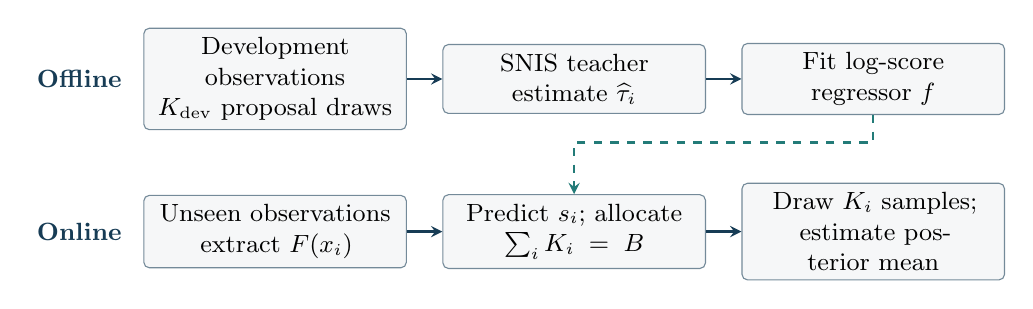
\begin{tikzpicture}[node distance=0.32cm, every node/.style={font=\small}, block/.style={draw=ink!60,rounded corners=2pt,minimum height=0.73cm,text width=3.1cm,align=center,fill=ink!4}, >=stealth]
\node[block] (a) {Development observations\\$\dev$ proposal draws};
\node[block,right=0.45cm of a] (b) {SNIS teacher\\estimate $\widehat\tau_i$};
\node[block,right=0.45cm of b] (c) {Fit log-score\\regressor $f$};
\draw[->,thick,ink] (a)--(b); \draw[->,thick,ink] (b)--(c);
\node[block,below=0.82cm of a] (d) {Unseen observations\\extract $F(x_i)$};
\node[block,right=0.45cm of d] (e) {Predict $s_i$; allocate\\$\sum_iK_i=B$};
\node[block,right=0.45cm of e] (g) {Draw $K_i$ samples;\\estimate posterior mean};
\draw[->,thick,ink] (d)--(e); \draw[->,thick,ink] (e)--(g);
\draw[->,thick,accent,dashed] (c.south) -- ++(0,-0.35) -| (e.north);
\node[anchor=east,font=\small\bfseries\color{ink}] at ([xshift=-0.15cm]a.west) {Offline};
\node[anchor=east,font=\small\bfseries\color{ink}] at ([xshift=-0.15cm]d.west) {Online};
\end{tikzpicture}
\captionof{figure}{Offline learning and online inference. No teacher sampling is required for a new observation.}
\end{center}
\subsection{Integer allocation and online inference}
In the implementation, $K_{\min}=4$ and $K_{\max}=120$. Reserve $K_{\min}$ draws per observation, and distribute the remaining budget according to the predicted scores. The continuous intermediate counts are
\begin{equation}
 k_i=K_{\min}+\min\{K_{\max}-K_{\min},\ c\,s_i\},\qquad\sum_i k_i=B,
\end{equation}
where $c$ is found by bisection. Floor the extra counts and assign residual draws in descending fractional-remainder order to eligible observations. This produces feasible integer counts and exactly preserves the budget. It is a stabilized, capped proportional-extras heuristic inspired by Eq.~\eqref{eq:optimal}, not the exact bounded optimum. Finally, apply Eq.~\eqref{eq:snis} using the allocated samples. Inference requires feature extraction and regression, but no online teacher draws. Offline costs are accounted for separately from online sampling costs.

\clearpage
\section{Completed study I: analytically tractable Gaussian mixtures}
\subsection{Model and evaluation design}
The synthetic model uses a two-component prior and a Gaussian observation model with context $c$ controlling the noise scale:
\begin{equation}
 p(z)=\sum_{j=1}^2\pi_j\N(z;m_j,I_d),\qquad p(x\mid z,c)=\N(x;z,\sigma_c^2 I_d),\quad d\in\{4,8\}.
\end{equation}
Completing the square gives a Gaussian-mixture posterior. Component $j$ has conditional mean $m_j'(x,c)=(x+\sigma_c^2m_j)/(1+\sigma_c^2)$ and covariance $\sigma_c^2 I_d/(1+\sigma_c^2)$. Its posterior weight is
\begin{equation}
 \gamma_j(x,c)=\frac{\pi_j\N(x;m_j,(1+\sigma_c^2)I_d)}{\sum_{\ell=1}^2\pi_\ell\N(x;m_\ell,(1+\sigma_c^2)I_d)}.
\end{equation}
Hence the exact posterior mean is $\mu(x,c)=\sum_j\gamma_j m_j'$. The marginal likelihood is
\[Z(x,c)=\sum_j\pi_j\N(x;m_j,(1+\sigma_c^2)I_d).\] The proposal is a single Gaussian; the exact posterior is not supplied to the learned predictor. The regressors receive $x$, $x^{\odot 2}$, $\norm{x}$, the proposal mean norm, proposal standard deviation, observation-noise standard deviation, and context index ($2d+5$ features).

\begin{center}
\small
\begin{tabularx}{\linewidth}{@{}lY@{}}
\toprule
Development & 800 observations per dimension; development seed 742; $\dev\in\{512,1024,2048\}$.\\
Pilot & Four held-out datasets (seeds 13, 37, 71, 101), 16 paired Monte Carlo trials each.\\
Confirmation & 25 new datasets per dimension (seeds 1001--1025); unchanged predictors; 16 trials each.\\
Online budget & 84 observations per dataset; 48 samples on average; $B=4032$.\\
Methods & Uniform, amortized ESS-derived allocation and task-aware allocation.\\
\bottomrule
\end{tabularx}
\captionof{table}{Synthetic experimental protocol. The 512-sample primary comparison was chosen after the pilot and checked on new datasets.}
\end{center}
The primary metric is $\MSE=\frac{1}{nd}\sum_i\norm{\widehat\mu_i-\mu_i}^2$; the secondary metric is $\frac1n\sum_i|\log\widehat Z_i-\log Z_i|$, where $\widehat Z_i=K_i^{-1}\sum_k w_{ik}$. For inference, average the paired trial differences within each dataset and then use dataset-level differences to calculate Student-$t$ intervals and sign-flip tests. Individual observations and Monte Carlo repetitions are not treated as independent datasets.
\subsection{Pilot and independent confirmation}
The four-dataset pilot found reductions of 11.65\% (4D) and 9.34\% (8D) at $\dev=512$. The exact two-sided sign-flip test had $p=0.125$ in both dimensions; the pilot was therefore not conclusive. The confirmation used the frozen predictors on new datasets. Its results are shown in Table~\ref{tab:synth}.
\begin{center}
\small
\begin{tabular}{@{}rr rrr rr@{}}
\toprule
$d$ & $\dev$ & Uniform & ESS-based & Task-aware & vs. uniform & vs. ESS\\
\midrule
4&512&0.087952&0.090669&0.079014&10.16\%&12.85\%\\
4&1024&0.087952&0.092471&0.079244&9.90\%&14.30\%\\
4&2048&0.087952&0.092113&0.079817&9.25\%&13.35\%\\
8&512&0.079915&0.081337&0.072789&8.92\%&10.51\%\\
8&1024&0.079915&0.082272&0.073244&8.35\%&10.97\%\\
8&2048&0.079915&0.082428&0.073349&8.22\%&11.01\%\\
\bottomrule
\end{tabular}
\captionof{table}{Per-coordinate posterior-mean MSE on the 25 confirmation datasets per dimension. The last two columns report relative error reductions.}\label{tab:synth}
\end{center}

\clearpage

\section{Completed study II: matched-budget baseline audit}\label{sec:baselines}
\subsection{Design and comparators}
The original 512-draw predictors were reconstructed from the same development seed (742), model, features and teacher code. I retained the original 25 confirmation datasets (1001--1025) and generated 25 fresh datasets (2001--2025) per dimension, with 84 observations and 16 paired trials per dataset. The original proposal is $q_i=\N(b_i,u_i I_d)$, where
\begin{equation}
 b_i=\frac{0.88x_i}{1+\sigma_{c_i}^2},\quad
 u_i=\frac{\sigma_{c_i}^2}{1+\sigma_{c_i}^2}\,a_{c_i}^{2},\quad
 (\sigma_c)=(0.45,1,2.1),\ (a_c)=(1,1.1,1.25).
\end{equation}
The mixture has weights $(0.55,0.45)$ and prior means $\pm 2.25 e_1$. Every method consumes exactly $B=4032$ density evaluations per trial and at most 120 per observation. Fixed-score policies share the same sample bank. Pilot policies use a separate eight-draw pilot bank and matched fresh draws; reuse requires $K_i\geq8$, and discard leaves 4--112 final draws per observation. The offline learned predictors consume 409,600 teacher evaluations per dimension, excluding model fitting.

\begin{center}\small
\begin{tabularx}{\linewidth}{@{}lY@{}}
\toprule
Method & Allocation score or rule\\
\midrule
Uniform & Equal counts, 48 draws per observation.\\
Amortized ESS; Learned task & Original fitted predictors, using weight variability or task-specific variance.\\
Context noise; Proposal width & $\sigma_c$ or $\sqrt{u_i}$; no training or pilot required.\\
Posterior-scale oracle & $\sqrt{\operatorname{tr}\operatorname{Cov}_{p_i}(z)}$, available analytically only here.\\
Variance oracles & Exact $\tau_i$ with original capped-extras rule or exact integer optimum.\\
Pilot8Fresh; Pilot8Reuse & Estimate the original teacher score from eight pilot draws. Discard or reuse these draws, counting them toward $B$.\\
Uniform pilot controls & Same pilot discard (40 fresh draws) or reuse (48 total draws) without adaptive allocation.\\
\bottomrule
\end{tabularx}
\captionof{table}{Baseline policies. Only oracle methods use analytic posterior information for allocation.}
\end{center}
\subsection{Results on original and fresh datasets}
\begin{center}\small
\begin{tabular}{@{}lrrrr@{}}
\toprule
&\multicolumn{2}{c}{Original confirmation}&\multicolumn{2}{c}{Fresh follow-up}\\
\cmidrule(lr){2-3}\cmidrule(l){4-5}
Method & 4D & 8D & 4D & 8D\\
\midrule
Context noise &11.89&10.30&\textbf{11.90}&\textbf{10.25}\\
Proposal width &11.28&10.24&11.45&10.18\\
Posterior-scale oracle &10.86&9.51&10.96&9.43\\
Learned task &10.16&8.92&10.45&8.88\\
Variance oracle (integer optimum)&6.84&5.59&6.50&5.48\\
Variance oracle (original rule)&6.58&5.47&6.34&5.31\\
Pilot8Reuse&6.09&2.60&5.10&2.85\\
Uniform&0&0&0&0\\
Uniform48ReusePilot&0.71&$-0.45$&$-0.94$&$-0.39$\\
Amortized ESS&$-3.09$&$-1.78$&$-3.99$&$-2.01$\\
Pilot8Fresh&$-8.20$&$-9.19$&$-8.95$&$-9.82$\\
Uniform40DiscardPilot&$-14.46$&$-14.13$&$-15.00$&$-14.48$\\
\bottomrule
\end{tabular}
\captionof{table}{Percentage reduction in posterior-mean MSE relative to uniform, with 25 datasets per dimension and cohort. Positive values favor the indicated method. The original learned results are reproduced, not counted as independent new evidence.}\label{tab:baselines}
\end{center}
\clearpage
\subsection{What the inexpensive baselines explain}
\begin{center}
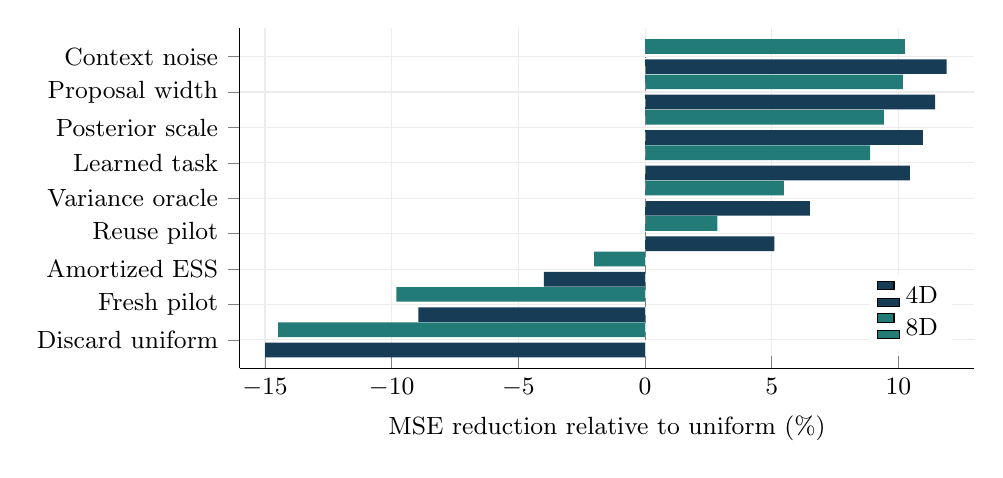
\begin{tikzpicture}
\begin{axis}[xbar,bar width=5.3pt,width=0.90\linewidth,height=5.9cm,xmin=-16,xmax=13,xtick={-15,-10,-5,0,5,10},ytick=data,symbolic y coords={Discard uniform,Fresh pilot,Amortized ESS,Reuse pilot,Variance oracle,Learned task,Posterior scale,Proposal width,Context noise},xlabel={MSE reduction relative to uniform (\%)},grid=major,grid style={gray!15},axis y line*=left,axis x line*=bottom,enlarge y limits=.10,tick label style={font=\small},label style={font=\small},legend style={at={(0.97,0.05)},anchor=south east,draw=none,font=\small}]
\addplot[fill=ink,draw=none] coordinates {(-15.00,Discard uniform)(-8.95,Fresh pilot)(-3.99,Amortized ESS)(5.10,Reuse pilot)(6.50,Variance oracle)(10.45,Learned task)(10.96,Posterior scale)(11.45,Proposal width)(11.90,Context noise)};\addlegendentry{4D}
\addplot[fill=accent,draw=none] coordinates {(-14.48,Discard uniform)(-9.82,Fresh pilot)(-2.01,Amortized ESS)(2.85,Reuse pilot)(5.48,Variance oracle)(8.88,Learned task)(9.43,Posterior scale)(10.18,Proposal width)(10.25,Context noise)};\addlegendentry{8D}
\draw[gray,dashed] (axis cs:0,Discard uniform)--(axis cs:0,Context noise);
\end{axis}
\end{tikzpicture}
\captionof{figure}{Fresh-cohort results reconstructed from the reported full-run summary (Table~\ref{tab:baselines}). The variance oracle is the exact bounded integer asymptotic optimum. Uniform is the zero reference.}
\end{center}
\begin{center}\small
\begin{tabular}{@{}llrrr@{}}
\toprule
$d$ & Paired contrast (learned minus baseline) & Difference & 95\% $t$ interval & Learned lower\\
\midrule
4 & Context noise & $+0.001242$ & $[0.000668,0.001817]$ &5/25\\
4 & Proposal width & $+0.000852$ & $[0.000538,0.001166]$ &3/25\\
8 & Context noise & $+0.001073$ & $[0.000653,0.001493]$ &4/25\\
8 & Proposal width & $+0.001018$ & $[0.000748,0.001289]$ &1/25\\
\bottomrule
\end{tabular}
\captionof{table}{Fresh datasets: paired differences in per-coordinate MSE. All four intervals exclude zero; positive differences favor the cheap rule. Monte Carlo sign-flip $p$-values range from 0.000020 to 0.000160.}\label{tab:cheap}
\end{center}
The original gain over uniform is reproducible: at $\dev=512$, the original paired 95\% intervals were $[-0.009609,-0.008266]$ (4D) and $[-0.007610,-0.006643]$ (8D). The learned method beat uniform and amortized ESS on all 25 original datasets at each teacher budget, but the learned component has no demonstrated advantage over the accessible heuristics. These results are conditional on the fitted predictors. Within-component posterior scale is $\sigma_c/\sqrt{1+\sigma_c^2}$, whose derivative is $(1+\sigma_c^2)^{-3/2}>0$. Context noise and proposal width are thus informative by construction; the full posterior also has between-component variance. The results are consistent with learning largely scale-related information, but do not identify the regressor's internal feature dependence.

The eight-draw pilot consumes 672 of 4032 evaluations. Discarding these draws leaves 3360 fresh draws; the adaptive fresh pilot nevertheless beats its uniform-40 control. Reusing pilot draws improves over uniform by 5.10\% and 2.85\% in the fresh cohort and beats its matched reuse control. Reuse changes the sampling rule adaptively and may alter finite-sample bias. The learned allocator beats both pilot variants, but neither amortization nor pilot sampling is universally preferable. This comparison tests sample counts, not total runtime or amortization break-even.
\clearpage
\section{Completed study III: exact asymptotic oracle and finite-sample risk}
\subsection{Analytical variance and oracle headroom}
For the synthetic model, the exact posterior has two Gaussian components with means $m_j'$ and common covariance $vI_d$, where $v=\sigma_c^2/(1+\sigma_c^2)$. To evaluate Eq.~\eqref{eq:tau} without noisy importance weights, expand $p(z)^2/q(z)$ into four Gaussian-product terms. Center coordinates at the proposal mean $b$, let $y=z-b$, $a_j=m_j'-b$, $t=\mu-b$, and $q=\N(b,u I_d)$. For each pair $(j,k)$, define
\begin{align}
 A&=2/v-1/u,\quad h_{jk}=(a_j+a_k)/v,\quad \ell_{jk}=h_{jk}/A,\\
 C_{jk}&=\frac{(2\pi u)^{d/2}}{(2\pi v)^d}\left(\frac{2\pi}{A}\right)^{d/2}
 \exp\!\left[-\frac12\left(\frac{\norm{a_j}^2+\norm{a_k}^2}{v}-\frac{\norm{h_{jk}}^2}{A}\right)\right].
\end{align}
Completing the square in $y$ gives a Gaussian with mean $\ell_{jk}$ and covariance $A^{-1}I_d$, multiplied by $C_{jk}$. Consequently,
\begin{equation}
 \boxed{\tau_i^2=\sum_{j,k}\gamma_j\gamma_k C_{jk}\left[d/A+\norm{\ell_{jk}-t}^{2}\right].}
\end{equation}
The integral is finite if $A>0$. Here $u=a_c^2v\geq v>0$, so this condition holds. In the exact-proposal case $q=p$, the score reduces to the trace of the posterior covariance. The notebook uses log-space accumulation and checks positivity and finiteness.

For equal observation weights, define the unrestricted continuous headroom
\begin{equation}
 G_{\rm cont}=1-\frac{J^*}{J_U}=1-\frac{(\sum_i\tau_i)^2}{n\sum_i\tau_i^2}
 =\frac{\operatorname{Var}_i(\tau_i)}{\operatorname{Var}_i(\tau_i)+\E_i[\tau_i]^2}.
\end{equation}
For the bounded integer problem, start at $K_i=4$ and successively assign one draw to the eligible observation with largest $\tau_i^2/[K_i(K_i+1)]$, stopping at the exact budget. This is optimal for the separable asymptotic objective because each marginal gain decreases with $K_i$. Let $J_O$ be this bounded optimum and $J_L$ the learned allocation's asymptotic risk. The captured fraction is $(J_U-J_L)/(J_U-J_O)$, using the same theoretical risk in all terms. The empirical oracle is evaluated separately with independent online draws, using the analytic posterior mean.
\begin{center}\small
\begin{tabular}{@{}lrrrr@{}}
\toprule
&\multicolumn{2}{c}{Original confirmation}&\multicolumn{2}{c}{Fresh follow-up}\\
\cmidrule(lr){2-3}\cmidrule(l){4-5}
Quantity (\%)&4D&8D&4D&8D\\
\midrule
Continuous asymptotic headroom&8.39&8.48&9.09&9.58\\
Bounded asymptotic headroom&8.37&8.45&9.06&9.46\\
Learned asymptotic headroom captured&37.11&28.55&32.73&25.29\\
Measured gain, bounded variance oracle&6.84&5.59&6.50&5.48\\
Measured gain, learned task&10.16&8.92&10.45&8.88\\
Measured learned/oracle gain ratio&148.61&159.53&160.84&162.10\\
\bottomrule
\end{tabular}
\captionof{table}{Oracle summary. Headroom and capture are ratios of cohort-mean asymptotic risks; the last three rows use measured finite-sample MSE. A ratio above 100\% in the last row does not violate the theoretical optimum: that oracle minimizes a different objective.}\label{tab:oracle}
\end{center}
\clearpage
\subsection{Testing the asymptotic approximation at operational budgets}
For each dimension, 12 observations per fresh dataset were randomly selected before risk inspection (300 observations from 25 datasets). For each observation I ran 1,024 independent SNIS repetitions, recording every prefix size $K=4,\ldots,120$ using the exact posterior mean. The nested prefixes share randomness across $K$ but each repetition is independent. Let
\begin{equation}
 R_i(K)=\frac1d\E\norm{\widehat\mu_{i,K}-\mu_i}^{2},\qquad
 \widehat R_i(K)=\frac{1}{1024d}\sum_{r=1}^{1024}\norm{\widehat\mu^{(r)}_{i,K}-\mu_i}^{2}.
\end{equation}
The theoretical prediction is $A_i(K)=\tau_i^2/(dK)$, and the calibration ratio is $C_i(K)=\widehat R_i(K)/A_i(K)$. The following plots use the nine reported sample counts from the full-run summary; the underlying experiment evaluated all 117 counts.
\begin{center}
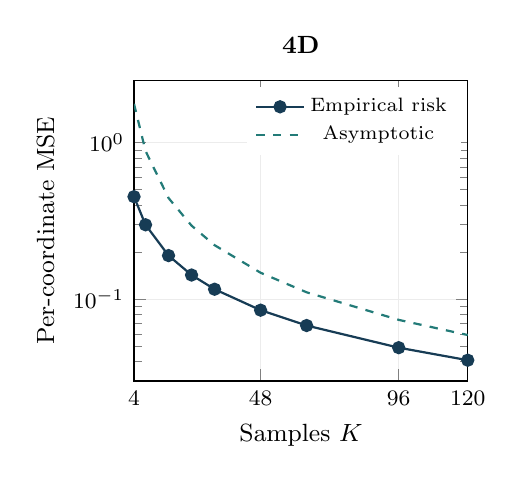
\begin{tikzpicture}
\begin{axis}[width=0.48\linewidth,height=5.4cm,xmin=4,xmax=120,xtick={4,48,96,120},xlabel={Samples $K$},grid=major,grid style={gray!15},tick label style={font=\footnotesize},label style={font=\small},title style={font=\small\bfseries},legend style={draw=none,font=\scriptsize,at={(0.98,0.98)},anchor=north east},title={4D},ymode=log,ymin=0.03,ymax=2.5,ylabel={Per-coordinate MSE}]
\addplot[ink,thick,mark=*] coordinates {(4,0.45178) (8,0.29878) (16,0.18995) (24,0.14268) (32,0.11575) (48,0.08507) (64,0.06787) (96,0.04900) (120,0.04075)};\addlegendentry{Empirical risk}
\addplot[accent,dashed,thick] coordinates {(4,1.77039) (8,0.88520) (16,0.44260) (24,0.29507) (32,0.22130) (48,0.14753) (64,0.11065) (96,0.07377) (120,0.05901)};\addlegendentry{Asymptotic}
\end{axis}
\end{tikzpicture}\hfill
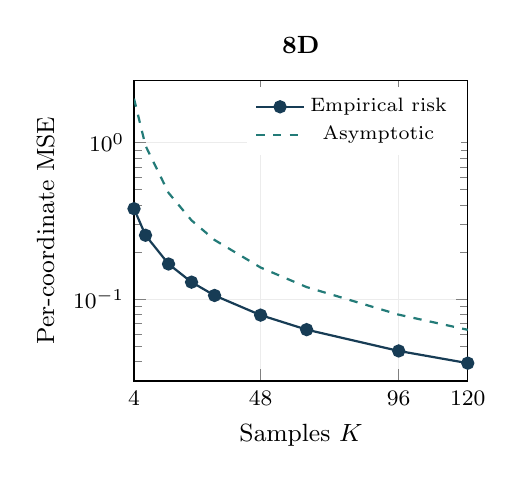
\begin{tikzpicture}
\begin{axis}[width=0.48\linewidth,height=5.4cm,xmin=4,xmax=120,xtick={4,48,96,120},xlabel={Samples $K$},grid=major,grid style={gray!15},tick label style={font=\footnotesize},label style={font=\small},title style={font=\small\bfseries},legend style={draw=none,font=\scriptsize,at={(0.98,0.98)},anchor=north east},title={8D},ymode=log,ymin=0.03,ymax=2.5,ylabel={Per-coordinate MSE}]
\addplot[ink,thick,mark=*] coordinates {(4,0.37856) (8,0.25606) (16,0.16781) (24,0.12846) (32,0.10562) (48,0.07912) (64,0.06388) (96,0.04670) (120,0.03903)};\addlegendentry{Empirical risk}
\addplot[accent,dashed,thick] coordinates {(4,1.91161) (8,0.95581) (16,0.47790) (24,0.31860) (32,0.23895) (48,0.15930) (64,0.11948) (96,0.07965) (120,0.06372)};\addlegendentry{Asymptotic}
\end{axis}
\end{tikzpicture}
\captionof{figure}{Mean empirical SNIS risk and exact asymptotic prediction, on randomly selected fresh observations. Both dimensions use the same logarithmic vertical scale. The theoretical curve substantially overestimates measured risk in the tested range.}\label{fig:risk}
\end{center}
\begin{center}\small
\begin{tabular}{@{}rr rrr rr@{}}
\toprule
$d$ & $K$ & Empirical MSE & Asymptotic MSE & Ratio of means & Median ratio & Spearman $\rho$\\
\midrule
4&4&0.45178&1.77039&0.25518&0.27212&0.78602\\
4&48&0.08507&0.14753&0.57660&0.61984&0.84202\\
4&120&0.04075&0.05901&0.69053&0.74354&0.84938\\
8&4&0.37856&1.91161&0.19803&0.24768&0.78962\\
8&48&0.07912&0.15930&0.49664&0.60640&0.78939\\
8&120&0.03903&0.06372&0.61248&0.74524&0.80727\\
\bottomrule
\end{tabular}
\captionof{table}{Selected finite-sample diagnostics. Ratio of means is distinct from median per-observation calibration; $\rho$ measures the association between empirical risk and $\tau_i^2$.}\label{tab:risk}
\end{center}
At $K=48$, the asymptotic prediction is about 1.73 times the measured mean risk in 4D and 2.01 times in 8D. Only 34 of 300 and 1 of 300 observations, respectively, have $0.8\leq C_i(48)\leq1.2$. Even at 120 draws, only 43\% and 35\% meet this criterion. These are empirical Monte Carlo risk estimates, not exact finite-sample integrals; their dispersion is assessed across observations rather than treated as independent confidence intervals.
\clearpage
\subsection{Calibration, task dependence and interpretation}
\begin{center}
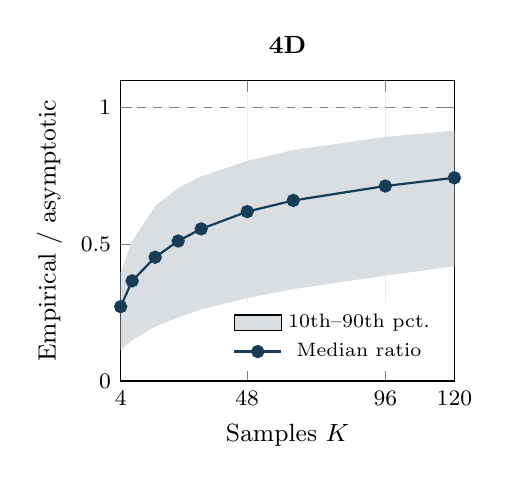
\begin{tikzpicture}
\begin{axis}[width=0.48\linewidth,height=5.4cm,xmin=4,xmax=120,xtick={4,48,96,120},xlabel={Samples $K$},grid=major,grid style={gray!15},tick label style={font=\footnotesize},label style={font=\small},title style={font=\small\bfseries},legend style={draw=none,font=\scriptsize,at={(0.98,0.98)},anchor=north east},title={4D},ymin=0,ymax=1.1,ylabel={Empirical / asymptotic},legend style={draw=none,font=\scriptsize,at={(0.97,0.03)},anchor=south east}]
\addplot[name path=lower,draw=none,forget plot] coordinates {(4,0.11345) (8,0.14925) (16,0.19929) (24,0.23244) (32,0.26197) (48,0.30330) (64,0.33644) (96,0.38553) (120,0.42005)};
\addplot[name path=upper,draw=none,forget plot] coordinates {(4,0.39724) (8,0.51265) (16,0.64001) (24,0.70656) (32,0.74872) (48,0.80553) (64,0.84528) (96,0.89330) (120,0.91587)};
\addplot[fill=ink!17,draw=none] fill between[of=lower and upper];\addlegendentry{10th--90th pct.}
\addplot[ink,thick,mark=*] coordinates {(4,0.27212) (8,0.36631) (16,0.45295) (24,0.51231) (32,0.55657) (48,0.61984) (64,0.66059) (96,0.71345) (120,0.74354)};\addlegendentry{Median ratio}
\addplot[gray,dashed,forget plot] coordinates {(4,1)(120,1)};
\end{axis}
\end{tikzpicture}\hfill
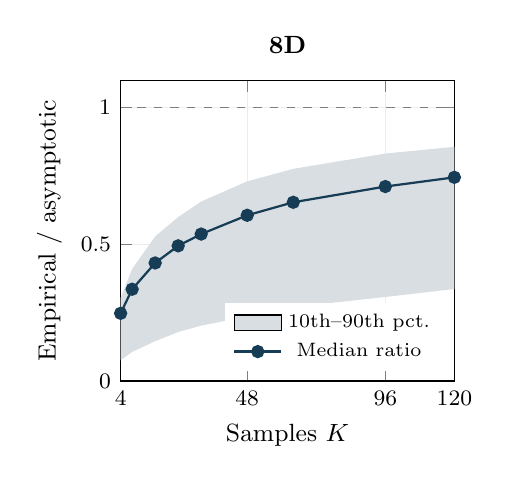
\begin{tikzpicture}
\begin{axis}[width=0.48\linewidth,height=5.4cm,xmin=4,xmax=120,xtick={4,48,96,120},xlabel={Samples $K$},grid=major,grid style={gray!15},tick label style={font=\footnotesize},label style={font=\small},title style={font=\small\bfseries},legend style={draw=none,font=\scriptsize,at={(0.98,0.98)},anchor=north east},title={8D},ymin=0,ymax=1.1,ylabel={Empirical / asymptotic},legend style={draw=none,font=\scriptsize,at={(0.97,0.03)},anchor=south east}]
\addplot[name path=lower,draw=none,forget plot] coordinates {(4,0.07574) (8,0.10641) (16,0.14573) (24,0.17931) (32,0.20268) (48,0.23632) (64,0.27068) (96,0.30743) (120,0.33666)};
\addplot[name path=upper,draw=none,forget plot] coordinates {(4,0.30404) (8,0.40995) (16,0.52914) (24,0.59973) (32,0.65669) (48,0.73043) (64,0.77624) (96,0.83228) (120,0.85686)};
\addplot[fill=ink!17,draw=none] fill between[of=lower and upper];\addlegendentry{10th--90th pct.}
\addplot[ink,thick,mark=*] coordinates {(4,0.24768) (8,0.33584) (16,0.43196) (24,0.49457) (32,0.53770) (48,0.60640) (64,0.65398) (96,0.71151) (120,0.74524)};\addlegendentry{Median ratio}
\addplot[gray,dashed,forget plot] coordinates {(4,1)(120,1)};
\end{axis}
\end{tikzpicture}
\captionof{figure}{Median empirical-to-asymptotic risk ratio and 10th--90th percentile band across observations, using reported full-run values at selected sample counts. The dashed line indicates exact calibration; bands are not confidence intervals.}\label{fig:cal}
\end{center}
The discrepancy is observation-dependent. If every risk were a common multiple of $\tau_i^2/K$, the same optimal allocation would follow. But the exact SNIS error has a random normalizer:
\begin{equation}
 R_i(K)=\frac1d\E_{q_i}\left[\frac{\norm{\sum_{k=1}^{K} w_{ik}(z_{ik}-\mu_i)}^2}{(\sum_{k=1}^{K}w_{ik})^2}\right].
\end{equation}
The numerator and denominator are dependent; finite-sample bias and rare weight events can distort the asymptotic approximation. The measured risk ratios vary substantially between observations, although the asymptotic score retains ranking information ($\rho=0.842$ and $0.789$ at 48 draws). The correct finite-budget objective depends on marginal changes in risk, not ranking alone. The exact asymptotic oracle is outperformed by the learned predictor and by cheap rules; this is evidence against treating the asymptotic objective as the finite-sample optimum, not against the asymptotic theorem itself.

\textbf{Task dependence and teacher cost.} In the original confirmation, 512-draw teachers gave 75\% fewer teacher density evaluations than 2048-draw teachers (409,600 vs. 1,638,400 per dimension), with no observed loss in posterior-mean accuracy. Each teacher budget uses one fitted predictor, so neither a general ranking nor a wall-clock saving follows. The task-aware method increased log-evidence MAE by 1.23--2.46\% across the six original settings. On fresh datasets the increase was 2.42\% and 2.06\% in 4D/8D; the ESS-derived allocator improved log-evidence MAE by only 0.12\% and 0.09\%. Context-noise allocation increased evidence MAE by 8.29\% and 8.77\%. Thus a policy that reduces posterior-mean error need not improve log evidence; the evidence does not show that the tested ESS policy is generally optimal for log evidence. In particular the asymptotic log-evidence variance $(\E_q[(p/q)^2]-1)/K$ is not itself an absolute-error objective.
\clearpage
\section{Completed study IV: transfer to learned generative models}
\subsection{VAE inference and independent reference checks}
The VAE defines a more realistic inference problem: $z\sim\N(0,I_d)$, $q_\phi(z\mid x)=\N(m_\phi(x),\operatorname{diag}(s_\phi^2(x)))$ and $p_\theta(x\mid z)=\N(g_\theta(z),\sigma_x^2 I)$ with $\sigma_x=0.15$. The $8\times8$ handwritten-digit images are from scikit-learn. The encoder and decoder are trained using the evidence lower bound \cite{kingma2014},
\begin{equation}
 \mathcal L_{\mathrm{ELBO}}=\E_{q_\phi}[\log p_\theta(x\mid z)]-\KL(q_\phi(z\mid x)\|p(z)).
\end{equation}
The frozen VAE defines the posterior; a separate regression model predicts the sampling difficulty, using pixel, encoder and reconstruction features. An initial three-seed 4D pilot was inconclusive. A 25-seed evaluation per dimension gave very small measured reductions (0.265\% and about 0.069\%). I then selected a temperature-scaled or defensive prior-mixture proposal using separate validation images:
\begin{equation}
 q_{T,\lambda}(z\mid x)=(1-\lambda)\N(z;m_\phi(x),T^2\operatorname{diag}(s_\phi^2(x)))+\lambda\N(z;0,I_d).
\end{equation}
Selection used median ESS fraction. For each dimension the follow-up used 25 trained VAEs, 104 previously unused test images, two groups of 52 with 2496 draws per group and 12 matched online repetitions. References pooled two independent 32,768-draw importance-sampling passes. The results below are measured against these approximate references.
\begin{center}\small
\begin{tabular}{@{}r rrr r r@{}}
\toprule
$d$ & Uniform MSE & Task MSE & Reduction & 95\% paired $t$ interval & Seeds lower\\
\midrule
4&0.014399&0.013689&4.93\%&$[-0.000900,-0.000521]$&25/25\\
8&0.106940&0.106029&0.85\%&$[-0.001583,-0.000239]$&17/25\\
\bottomrule
\end{tabular}
\captionof{table}{Selected-proposal task-aware versus uniform, using approximate IS references.}
\end{center}
The reference ESS fraction was below 1\% for 17.8\% and 53.9\% of reference observations. A 4D audit found one draw carrying 83.17\% of normalized weight despite 131,072 samples; independent repeats produced another extreme-weight event. Let $\mu_{\rm ref}=\mu+\delta$, and let $\widehat\mu_T,\widehat\mu_U$ be the two estimates. Then the measured paired squared-error difference is
\begin{equation}
 \Delta_{\rm ref}=\norm{\widehat\mu_T-\mu}^2-\norm{\widehat\mu_U-\mu}^2-2(\widehat\mu_T-\widehat\mu_U)^\top\delta.
\end{equation}
The cross term can distort a small effect. I therefore used HMC \cite{neal2011} as an alternative reference, sampling from the posterior with potential $U(z)=\norm z^2/2+\norm{x-g_\theta(z)}^2/(2\sigma_x^2)$. On a fixed exploratory subset of eight 8D VAEs and twelve images, 93 of 96 cases passed basic diagnostics (rank-normalized $\widehat R<1.01$, bulk ESS $>400$, acceptable integration and acceptance checks \cite{vehtari2021}). Four chains used 1,000 warmup and 2,000 retained draws each. Original allocations were frozen; the subset was not reallocated.
\begin{center}\small
\begin{tabular}{@{}lrrrr@{}}
\toprule
Reference (matched subset)&Uniform&Task&Reduction&Sign-flip $p$\\
\midrule
HMC, all chains&0.123149&0.122539&0.495\%&0.6953\\
HMC, chains 1--2&0.122436&0.121907&0.432\%&0.7344\\
HMC, chains 3--4&0.123990&0.123300&0.557\%&0.6563\\
Original IS&0.122121&0.121679&0.362\%&0.7734\\
\bottomrule
\end{tabular}
\captionof{table}{Seed-level comparison on diagnostically passing cases, eight seeds. Chain groups are reference sensitivity checks, not independent allocation experiments.}
\end{center}
The all-chain paired difference was $-0.000610$, 95\% interval $[-0.004387,0.003168]$, with five of eight seeds favoring the task allocator. The interval is wide relative to the observed effect; HMC does not establish a reliable improvement. Low ESS motivates proposal repair rather than simply allocating more draws, but 1\% is a diagnostic threshold, not a universal impossibility bound. Further work will prioritize tractable posterior references rather than more VAE reference forensics.
\clearpage
\section{Research hypotheses and proposed work}\label{sec:future}
The completed studies show two distinct limitations: the original ML score did not exceed the cheap scale baselines, and even exact asymptotic difficulty did not determine the best finite-budget allocation. I propose to investigate them together. The following experiments are future work, not results.
\subsection{H1: Learning finite-sample risk beyond accessible scale}
\textbf{Hypothesis.} When posterior geometry and proposal mismatch vary beyond what accessible scale features explain, a finite-sample risk predictor can improve on inexpensive deterministic allocation and the learned asymptotic score. The target is $R_i(K)$, not a scalar variance proxy. I will estimate empirical risk curves on separate development data, fit a positive model $\widehat R_\psi(F(x_i),K)$ and select integer counts by
\begin{equation}
 \min_{K_i\in\{4,\ldots,120\}}\sum_i\widehat R_\psi(F(x_i),K_i),\qquad \sum_i K_i=B.
\end{equation}
A dynamic program can solve the separable discrete problem without assuming monotonic marginal gains. With $D_j(b)$ the minimum predicted risk of allocating $b$ samples to the first $j$ observations,
\begin{equation}
 D_j(b)=\min_{4\leq k\leq120}\{D_{j-1}(b-k)+\widehat R_\psi(F(x_j),k)\},\quad D_0(0)=0,
\end{equation}
with other infeasible states set to infinity. Backtracking recovers the allocation. If diminishing marginal risk reductions are verified, a greedy allocator can be compared as a cheaper approximation.

I will first construct a finite-sample oracle by estimating risk curves on test observations using a large independent simulation bank, optimize the estimated curves, and evaluate the chosen allocations on a second bank to avoid selection bias. The oracle is a privileged, approximate benchmark; its evaluation cost is not included as an online method. The learned predictor will use only development curves, and be compared with uniform, context noise, proposal width, pilot reuse and the original asymptotic learned allocator. A scale-only risk model and ablations of context and proposal features will test whether learning adds information beyond scale. With multiple development seeds, I will measure paired test MSE and the incremental gain over the best prespecified cheap baseline, not merely over uniform.
\subsection{H2: Reliability-aware allocation under proposal mismatch}
\textbf{Hypothesis.} Validation-based calibration and shrinkage reduce harmful reallocations when learned risk curves are unreliable. Let $K_i^L$ be the learned finite-risk allocation and $K_i^0$ a cheap baseline fixed using development/validation data. Define a continuous blend before integerization:
\begin{equation}
 k_i(\alpha)=(1-\alpha)K_i^0+\alpha K_i^L,\qquad 0\leq\alpha\leq1.
\end{equation}
Both endpoint allocations are feasible, so the blend preserves the budget and bounds; largest-remainder rounding preserves the exact integer total. The fallback can be uniform or a selected scale rule. The blend coefficient is chosen on independent validation batches using risk calibration, disagreement across teacher runs, and proposal-derived indicators available without extra sampling. If a pilot diagnostic is used, its evaluations are charged to the online budget. I will compare fixed shrinkage with validation-calibrated shrinkage and report the frequency and magnitude of harmful allocation, not only the mean gain. Shrinkage is not a substitute for a reliable proposal: under severe mismatch, proposal adaptation is a separate intervention whose costs must be reported.
\clearpage
\subsection{A nonlinear test with tractable reference means}
A two-dimensional nonlinear synthetic model will separate posterior geometry from uncertainty due to reference estimation:
\begin{equation}
 z\sim\N(0,I_2),\quad x=g(z)+\epsilon,\quad \epsilon\sim\N(0,\sigma^2 I_2),\quad
 g(z)=\begin{bmatrix}z_1^2+0.5z_2\\\sin(z_1)+z_2\end{bmatrix}.
\end{equation}
This model can produce non-Gaussian posteriors. I will calculate reference means by integrating the unnormalized posterior on a numerical grid,
\begin{equation}
 \mu(x)=\frac{\int z\exp[-\norm z^2/2-\norm{x-g(z)}^2/(2\sigma^2)]\,dz}
 {\int\exp[-\norm z^2/2-\norm{x-g(z)}^2/(2\sigma^2)]\,dz},
\end{equation}
and test accuracy through domain expansion and grid refinement, with thresholds set before final evaluation. This is a converged numerical reference rather than an exact analytic mean. Proposal means and widths will be varied in a controlled manner, including an explicitly defensive mixture. The test will distinguish cases with similar accessible proposal scale but different posterior geometry. This is the setting in which a learned predictor has an opportunity to add value beyond context noise or width.

\textbf{Evaluation safeguards.} Development, validation and final test datasets will be disjoint. The proposal menu, teacher budgets, sample bounds, primary comparison, reference tolerances and reporting rules will be fixed before final tests. The unit of uncertainty is the independent dataset or fitted-model seed, not individual Monte Carlo draws. I will report paired confidence intervals and the distribution of gains under matched sample budgets, including failures and reference coverage. Predicted risk calibration, marginal risk errors and finite-sample oracle headroom will be evaluated separately. Comparisons that select an oracle or a policy using estimated risks must be evaluated on independent draws. If the learned predictor does not beat a cheap baseline, that negative result will be retained.
\section{Scope, expected contribution and conclusion}
The underlying SNIS variance and continuous resource-allocation rule are established mathematical principles \cite{owen2013}. Prior work on importance-weighted variational learning \cite{burda2016,rainforth2018,tucker2019} motivates the distinction between sampling, statistical objectives and model learning; it does not by itself establish novelty for the proposed allocation approach. A broader literature comparison is part of the future work.

The strongest completed evidence is now more specific than the original improvement over uniform: the learned allocator reproduces its synthetic gain but does not outperform cheap scale rules, and the exact asymptotic optimum is not the best tested finite-budget policy. The finite-sample risk audit establishes substantial miscalibration in the range actually used for inference, while the VAE studies demonstrate how reference error and proposal quality complicate evaluation. The proposed research therefore focuses on learning risk when simple information is insufficient and recognizing when a simpler allocation is preferable. Generalization to other posterior statistics and a full amortized runtime cost model are valuable extensions, but are outside the primary scope.

The expected contribution is a principled and experimentally testable account of when learning can improve finite-budget posterior inference beyond inexpensive allocation rules, with reliable baselines, a finite-sample oracle, and calibrated fallback policies. The goal is not to claim improvement universally, but to establish the conditions under which the extra learning effort is justified.
\clearpage
\section*{Reproducibility and supporting experimental records}
The original synthetic studies use the Phase 2 notebook and its 512/1024/2048 teacher-budget trial and confirmation files. The 2026 synthetic oracle-and-risk follow-up notebook uses the same generator and 512-draw training procedure. The original confirmation seeds are 1001--1025 and the fresh seeds are 2001--2025. The full-run outputs are: \path{baseline_summary.csv}, \path{paired_comparisons.csv}, \path{oracle_summary.csv}, \path{finite_sample_risk_summary.csv}, and the per-observation risk CSV. The new figures reproduce the numerical summaries supplied from the full run; the risk figures use selected reported sample counts. No new simulation results were generated for this document. The per-coordinate metric is already averaged across latent coordinates and is not divided by $d$ again.

The VAE study uses the separate confirmation, proposal-follow-up and reference-audit notebooks. The direct HMC comparison is recorded in \path{hmc_coverage_by_seed.csv} and \path{seed_level_hmc_comparisons.csv}. Its seeds are 27002, 27003, 27008, 27011, 27015, 27018, 27020, 27022; the image indices within the fixed follow-up set are 2, 19, 26, 34, 40, 44, 48, 65, 66, 71, 88, 90. The HMC reference is approximate and the tested subset does not constitute a new independent VAE training experiment. The bibliography below is retained from the preceding version, with sources published through 2021.
\begin{thebibliography}{9}
\bibitem{owen2013} A. B. Owen. \emph{Monte Carlo Theory, Methods and Examples}. 2013. \url{https://artowen.su.domains/mc/}.
\bibitem{kingma2014} D. P. Kingma and M. Welling. Auto-encoding variational Bayes. \emph{International Conference on Learning Representations}, 2014. \url{https://arxiv.org/abs/1312.6114}.
\bibitem{burda2016} Y. Burda, R. Grosse, and R. Salakhutdinov. Importance weighted autoencoders. \emph{International Conference on Learning Representations}, 2016. \url{https://arxiv.org/abs/1509.00519}.
\bibitem{rainforth2018} T. Rainforth et al. Tighter variational bounds are not necessarily better. \emph{Proceedings of the 35th International Conference on Machine Learning}, 2018. \url{https://proceedings.mlr.press/v80/rainforth18b.html}.
\bibitem{tucker2019} G. Tucker, D. Lawson, S. Gu, and C. J. Maddison. Doubly reparameterized gradient estimators for Monte Carlo objectives. \emph{International Conference on Learning Representations}, 2019. \url{https://arxiv.org/abs/1810.04152}.
\bibitem{neal2011} R. M. Neal. MCMC using Hamiltonian dynamics. In \emph{Handbook of Markov Chain Monte Carlo}, Chapman and Hall/CRC, 2011. \url{https://arxiv.org/abs/1206.1901}.
\bibitem{vehtari2021} A. Vehtari, A. Gelman, D. Simpson, B. Carpenter, and P.-C. B\"urkner. Rank-normalization, folding, and localization: An improved $\widehat R$ for assessing convergence of MCMC. \emph{Bayesian Analysis}, 16(2):667--718, 2021. \url{https://doi.org/10.1214/20-BA1221}.
\end{thebibliography}
\end{document}
